\documentclass[a4paper,12pt]{article}

\usepackage[lmargin=2.5cm,rmargin=2.5cm,tmargin=2.5cm,bmargin=1.5cm,includefoot]{geometry}
\usepackage[T1]{fontenc}
\usepackage[utf8]{inputenc}
\usepackage{times}
\usepackage[colorlinks,linkcolor=blue,citecolor=blue,urlcolor=blue]{hyperref}
%\usepackage[french]{babel}
\usepackage{xargs}
\usepackage{amssymb,amsfonts,amsthm,amsmath}
\usepackage{graphicx}
\usepackage{xcolor}
\usepackage{marvosym}
\usepackage{pdfpages}
\usepackage{xcolor}
\usepackage{paralist}
\graphicspath{{figures/}}



% math special letters
\newcommand{\R}{\mathbb{R}} % reals
\newcommand{\N}{\mathbb{N}} % naturals
\newcommand{\Z}{\mathbb{Z}} % integers
\newcommand{\I}{\mathbb{I}} % set of integers
\newcommand{\C}{\mathbb{C}} % set of summands
\newcommand{\cA}{\mathcal{A}} % algebra
\newcommand{\cL}{\mathcal{L}} % algebra
\newcommand{\cG}{\mathcal{G}} % Grotendick group
\newcommand{\fA}{\mathfrak{A}} % alternating group
\newcommand{\fS}{\mathfrak{S}} % symmetric group
\newcommand{\HH}{\mathbb{H}} % hyperplane
\renewcommand{\b}[1]{\mathbf{#1}} % bold letters

% math commands
\newcommand{\set}[2]{\left\{ #1 \;\middle|\; #2 \right\}} % set notation
\newcommand{\bigset}[2]{\big\{ #1 \;|\; #2 \big\}} % big set notation
\newcommand{\biggset}[2]{\bigg\{ #1 \;\bigg|\; #2 \bigg\}} % big set notation
\newcommand{\multiset}[2]{\left\{\!\!\left\{ #1 \;\middle|\; #2 \right\}\!\!\right\}} % multiset notation
\newcommand{\bigmultiset}[2]{\big\{\!\!\big\{ #1 \;|\; #2 \big\}\!\!\big\}} % big multiset notation
\newcommand{\ssm}{\smallsetminus} % small set minus
\newcommand{\dotprod}[2]{\langle #1 | #2 \rangle} % dot product
\newcommand{\symdif}{\, \triangle \, } % symmetric difference
\newcommand{\one}{{1\!\!1}} % the all one vector
\newcommand{\eqdef}{\mbox{\,\raisebox{0.2ex}{\scriptsize\ensuremath{\mathrm:}}\ensuremath{=}\,}} % :=
\newcommand{\defeq}{\mbox{~\ensuremath{=}\raisebox{0.2ex}{\scriptsize\ensuremath{\mathrm:}} }} % =:
\newcommand{\polar}{^\diamond} % polar
\newcommand{\simplex}{\triangle} % simplex
\newcommand{\defn}[1]{\emph{\color{blue} #1}} % emphasis of a definition

\newcommand{\Ind}[2]{\mathrm{Ind}_{{#1}}^{{#2}}}
\newcommand{\Sym}{\mathsf{Sym}} % symmetric functions
\newcommand{\FQSym}{\mathsf{FQSym}} % quasi-symmetric functions
\newcommand{\PBT}{\mathsf{PBT}} % Planar binary tree algebra
\newcommand{\Camb}{\mathsf{Camb}} % Cambrian algebra
\newcommand{\Rec}{\mathsf{Rec}} % recoils algebra
\newcommand{\NCSF}{\mathsf{NCSF}} % NCSF algebra
\newcommand{\FSym}{\mathsf{FSym}} % FSym
\newcommand{\QSym}{\mathsf{QSym}} % FSym
\newcommandx{\Asso}[1][1=n]{\mathsf{Asso}(#1)} % associahedron
\newcommandx{\Perm}[1][1=n]{\mathsf{Perm}(#1)} % permutahedron
\newcommandx{\Para}[1][1=n]{\mathsf{Para}(#1)} % parallelepiped
\newcommand{\red}{\color{red}} % red command
\newcommand{\blue}{\color{blue}} % blue command

\newcommand{\includeSymbol}[1]{\ensuremath{%
	\mathchoice
		{\raisebox{-.7mm}{\includegraphics[height=2.2ex]{#1}}}	
		{\raisebox{-.7mm}{\includegraphics[height=2.2ex]{#1}}}
		{\raisebox{-.6mm}{\includegraphics[height=1.6ex]{#1}}}
		{\raisebox{-.5mm}{\includegraphics[height=1ex]{#1}}}
}}
\newcommand{\noneCirc}{\includeSymbol{none}}
\newcommand{\upCirc}{\includeSymbol{up}}
\newcommand{\downCirc}{\includeSymbol{down}}
\newcommand{\upDownCirc}{\includeSymbol{updown}}
\newcommand{\Decorations}{\{\noneCirc{}, \downCirc{}, \upCirc{}, \upDownCirc{}\}} % all decorations
\newcommandx{\Permutreehedron}[1][1=\delta]{\mathsf{PT}(#1)} % permutreehedron

\usepackage{todonotes}
\newcommand{\vincent}[1]{\todo[color=blue!30]{#1}}
\newcommand{\viviane}[1]{\todo[color=red!30]{#1}}



\title{\huge \bf ???  \\ Combinatorics, Algebra, and Geometry \\ from Cambrian to Permutree lattices}
\author{Viviane Pons, Vincent Pilaud, Florent Hivert}
\date{April 2019}

\begin{document}
\maketitle

\section{Presentation}

This thesis is within the range of algebraic and geometric combinatorics. We study classical structures of computer science such as \emph{partial orders} and \emph{lattices} over combinatorial objects. These are related to algebraic structures such as Hopf algebras and to geometrical objects such as polytopes and reflection groups. Thus we are interfacing between combinatorics, algorithmic, geometry and algebraic computation.

More specifically, we are interested in the Tamari lattice on binary trees~\cite{Tamari, HuangTamari, TamariFestschrift}, in the weak order on permutations, and in some of their generalizations. The Cambrian lattices~\cite{Reading-cambrianLattices} have been introduced recently by Reading as generalization of the Tamari lattice. In particular, their definition is related to finite Coxeter groups~\cite{Reading-FiniteCoxeterGroupsChapter}. On the other hand, Piland and Pons have described the Permutree lattices~\cite{PilaudPons-permutrees}, which interpolate between the weak order on permutations, the Tamari lattice, and the boolean lattice. In particular, the Cambrian lattices attached to the finite Coxeter group of type $A$ are a special case of permutree lattices. The goal of this thesis is to understand the relation between the Permutree lattices and the finite Coxeter groups, \emph{i.e.} how to define the Permutree lattices for finite Coxeter groups other than type $A$? More generally, we want to survey all existing results on Cambrian lattices and see which ones can be extended to Permutree lattices. On the combinatorial side, it will give us a good comprehension of the lattice quotient and sublattices of the weak order in all types. On the geometrical side, it might lead to the definition of new polytopes. And on the algebraic side, we might obtain new Hopf algebras or related structures.

\section{Thematic and context}

\subsection{Coxeter groups and Cambrian lattices}

\subsection{Permutree lattices}

The permutree lattices~\cite{PilaudPons-permutrees} are an interpolation between three famous structures (see Fig.~\ref{fig:classicalLattices}):

\begin{compactitem}
\item the \defn{weak order} on permutations of~$\fS_n$, defined as the inclusion of inversion sets,
\item the \defn{Tamari lattice} on binary trees with $n$ nodes, defined as the transitive closure of right rotations,
\item the \defn{boolean lattice} on binary sequences with $n-1$ letters.
\end{compactitem}
The Tamari lattice is a fundamental combinatorial tool introduced by D.~Tamari in~\cite{Tamari}, and has motivated a wide variety of research directions since then.
An overview of these research topics is available in the survey book~\cite{TamariFestschrift}.
One way to see that it is a lattice is to see it as a lattice quotient of the weak order~\cite{Reading-cambrianLattices, ChatelPilaud}.

\begin{figure}[h]
	\centerline{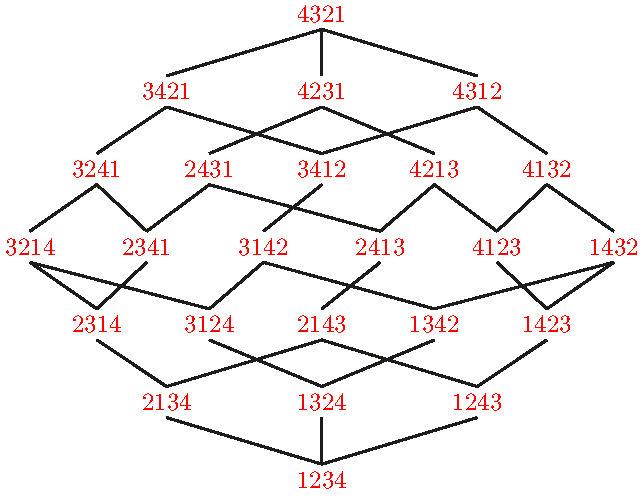
\includegraphics[scale=.55]{weakOrder}\qquad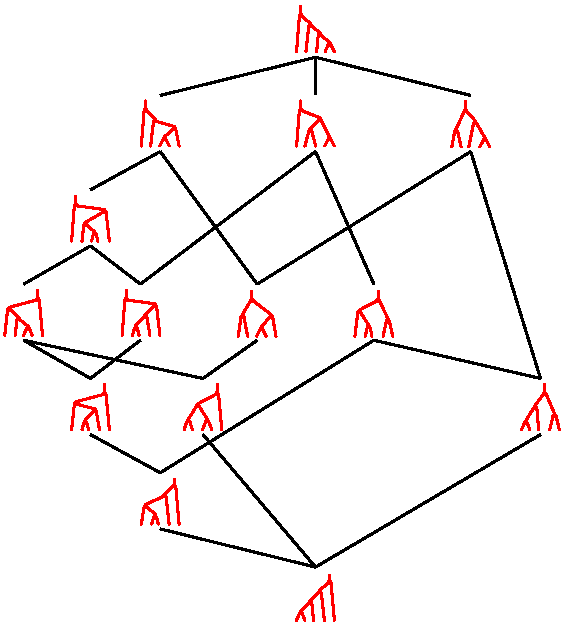
\includegraphics[scale=.45]{TamariLattice}\qquad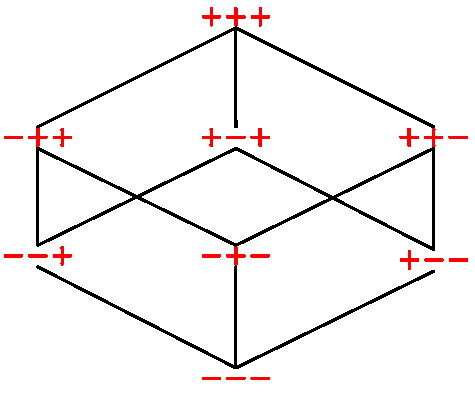
\includegraphics[scale=.7]{booleanLattice}}
	\caption{The weak order (left), the Tamari lattice (middle) and the boolean lattice (right).}
	\label{fig:classicalLattices}
\end{figure}

\begin{figure}[h]
	\centerline{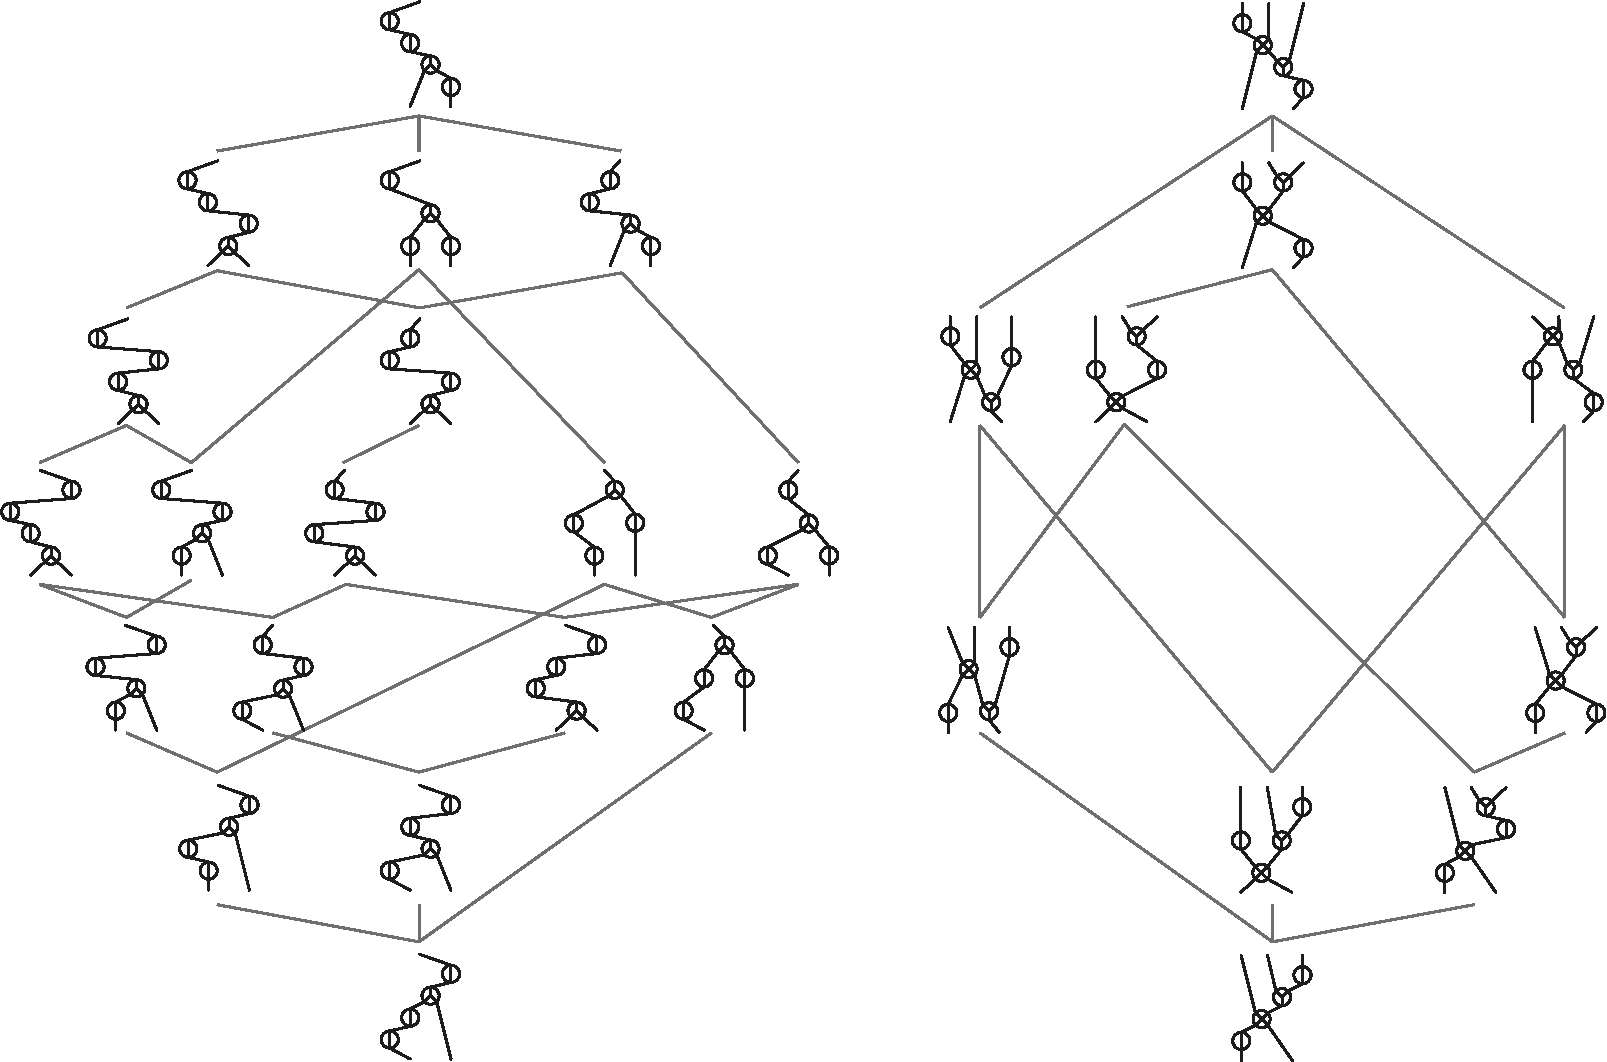
\includegraphics[scale=.5]{permutreeLattices}}
	\caption{Some permutree lattices (right).}
	\label{fig:permutreeLattices}
\end{figure}

Given a decoration~$\delta \in \Decorations^n$, a \defn{$\delta$-permutree}~\cite{PilaudPons-permutrees} is an oriented and labeled tree such that the node labeled~$i$ has one or two parents and one or two children depending on~$\delta_i$, and with local conditions on the labeling.
Permutrees should be consider as hybrid combinatorial objects between permutations (obtained when each node has one parent and one child), binary trees (obtained when each node has one parent and two children), and binary sequences (obtained when each node has two parents and two children).
%The $\delta$-permutrees correspond to the vertices of a polytope~$\Permutreehedron$ called \defn{permutreehedron}~\cite{PilaudPons-permutrees}.
There is also a natural rotation operation on $\delta$-permutrees, with a natural orientation, and the transitive closure of this operation defines a lattice on $\delta$-permutrees called \defn{permutree lattice} and denoted~$\cL(\delta)$.
See Fig.~\ref{fig:permutreeLattices}.
For example, the weak order on permutations is the permutree lattice~$\cL(\noneCirc^n)$, the Tamari lattice is the permutree lattice~$\cL(\downCirc^n)$, and the boolean lattice is the permutree lattice~$\cL(\upDownCirc^n)$.
The permutree lattice is always a lattice quotient of the weak order on permutations.

\viviane{Add something about polytopes and Hopf algebras}

\subsection{Specific context of the thesis}

As previously described, we have two families of interesting structures, the Cambrian lattices and the Permutree lattices, both generalizing the Tamari lattice. They overlap in the sense that the Cambrian lattices of type $A$ are a specific case of Permutree lattices. They correspond to a decoration $\delta \in \lbrace \upCirc, \downCirc \rbrace^n$. The problem of defining Permutree lattices for other types has never been studied and raises many interesting questions:

\begin{compactitem}
\item Each permutree can be injectively sent to a couple of permutations. In type $A$, these permutations can be characterized through pattern avoidance. Can we also characterize them by conditions on their reduced words as elements of the type $A$ Coxeter group? 
\item Can this characterization be generalized to other types? Do they also give sublattices of the weak order?
\item What would be the combinatorial description of permutrees in other types?
\item Do permutree in other types lead to the definition of new polytopes?
\item Can we define Hopf algebras in other types?
\end{compactitem}

We have good reasons to believe that some of these questions have positive answers and lead to very interesting research and results. 
\viviane{Add a word about it being a trending topic, cite other stuff on the Tamari lattice}

\section{Objectives, method and expected results}

\subsection{Objectives}

\subsection{Method}

The project can be done in 3 phases.

In phase one, the candidate must familiarize themselves with the notions at play: the different lattice structures, the finite Coxeter groups, the Permutree lattices, and the Cambrian lattices. They must gain a fine understanding of their interactions and be able to easily experiment and explore.

In phase two, they will try to better understand the relation between Permutrees and the type $A$ Coxeter group in order to generalize some results to other classical types such as $B$ and $D$. 

In phase three, they will try to obtain some generic results and proof for all types and understand which properties of Cambrian lattices can be extended to all types Permutrees and why. 

\subsection{Computer exploration and SageMath}

Florent Hivert and Viviane Pons are two active contributors to the open-source mathematical software SageMath (see \url{http://www.sagemath.org}). Florent Hiver, along with Nicolas Thiéry, was the initiator of a development project for experimental combinatorial research. The project was first developed on the computational system MuPAD before moving to SageMath in 2008 as Sage-Combinat. In 2015, the success of the SageMath community has been recognized and supported by the European Union through the OpenDreamKit (see \url{https://opendreamkit.org/}) H2020 grant: Open Digital Research Environment Toolkit for the Advancement of Mathematics. The coordinator of the project is Nicolas Thiéry (LRI, Paris-Sud). Florent Hivert and Viviane Pons are both members and Viviane Pons is the local coordinator for Paris-Sud as well as the work package leader of \emph{Community Building, Training, Dissemination, Exploitation, and Outreach}. In partcular, she has been giving many SageMath lectures, tutorials and workshops around the academic world and has organized many SageMath events.

SageMath is an open-source mathematical software under the GPL license. It combines the functionalities of many open-source software under a common interface based on the programming language python. It covers a vast range of mathematics including algebra, analysis, number theory, cryptography, numerical analysis, commutative algebra, group theory, combinatorics, graph theory, formal linear algebra, etc. The combinatorician community is particularly active, developing what is known as Sage-Combinat, whose mission is to ``to improve the open-source mathematical system Sage as an extensible toolbox for computer exploration in (algebraic) combinatorics, and foster code sharing between researchers in this area''. Sage-Combinat is gathering about fifty international contributors (Europe, North America, Australia, Japan, Korea, ...).

This research will strongly rely on computer exploration and mathematical experimentation. This methodology is used and promoted by all three advisers as demonstrated by the recent interventions of Viviane Pons in the python community such as her talk ``Experimental pure mathematics using Sage'' at PyCon 2015 and her keynote presentation ``Science and open-source: what do we learn from each other?'' at PyConFr 2018. The main tool will be the software SageMath. This will allow the student to join an international development team and to gain an experience in collaborative development and computer exploration. This will be very valuable for their future career. 


\subsection{Expected results}

\begin{compactitem}
\item publications in international journals recognized by the community (JCTA, ALCO, EJC, etc.);
\item publications in international conferences of the domain (FPSAC, EuroComb);
\item presentations in national and international workshops of the domain;
\item contributions to the sofwatre SageMath.
\end{compactitem}

\section{Scientific environment}

\subsection{Scientific and material conditions}

The thesis will take place in the GALaC team of LRI with a strong connection to the combinatorics team of LIX. The student will benefit from an active research environment with many other students working on similar subjects: 8 students (Master internships, PhD students, visiting students) working on combinatorics between GALaC and LIX this semester. A joint combinatorics seminar is organized weekly between GALaC and LIX as well as a team seminar in GALaC (at least once per month). They will also benefit from the rich combinatorial research environment of the Paris area: Flajolet seminar at IHP every two months, discrete geometry seminar at IHP, student seminar at IHP (co-organized by Justine Falque from GALaC). 

\subsection{International opportunities}

All three advisors have strong international collaborations going on, especially in Europe and North America. Viviane Pons has been leading a PHC Amadeus project with Vienna (Austria) for the past 18 months. This will give a direct opportunity for the student to travel to Vienna and present their results at the University of Vienna and Technichal University of Vienna. Vincent Pilaud is also part of this project, which is based on a long standing collaboration between Cesar Ceballos in Vienna and both Vincent Pilaud and Viviane Pons in France. 

We also have on going collaborations with researchers from Canada, especially Nantel Bergeron in Toronto (York University) and François Bergeron in Montréal (LACIM, UQAM). François Bergeron has been a visiting professor in GALaC for the past year. All three advisors are associated members of the CNRS international department LIRCO (UQAM, Montréal), which offer great travel opportunities to students. 

Finally, Viviane Pons and Vincent Pilaud have a strong connection to Colombia. Vincent Pilaud has been an organizer of the ECCO (Encuentro Colombiano de Combinatoria) summer school, supported by the CIMPA program, in 2018 in Barranquilla and in 2016 in Medellin. Viviane Pons was an invited professor both times to organize the SageMath tutorials. She will be an organizer of the 2020 edition in Bogota (in charge of the CIMPA funding). The 2020 ECCO in Bogota will be the 7th edition of the school, which gathers between 100 and 200 students from all over the world (from undergrads to postdocs). Over the years, it has gained a solid reputation in the international community both from its high scientific quality and for the role it plays in connecting students from South America to the global academic world. 

\subsection{Possible collaboration}

\subsection{Valorization objectives}

\section{Candidate profile}

We expect the candidate to have already a good background in combinatorics with a strong understanding of the objects at play such as lattices and polytopes. The candidate must have carried a research project or internship in the domain. They must have some experience of programming.

\bibliographystyle{alpha}
\small
\renewcommand{\refname}{\normalsize Bibliography}
\bibliography{projetStage}
\normalsize

\end{document}
